\begin{itemize}
    \item Diagnostic X-Ray Machine
    \item X-Ray QA Kit. (Equipment Details given below)
\end{itemize}
\subsection{Cobia Smart R/F}
The Cobia Smart R/F is a user-friendly, all-in-one X-ray QA (Quality Assurance) meter from RTI Group designed for straightforward testing of conventional radiography and fluoroscopy units, as well as intraoral dental and CBCT systems. It provides instant and accurate readings of key X-ray parameters without requiring user adjustments. 

\subsection{RTI Scatter Probe}
The RTI Scatter Probe is a rugged, solid-state detector designed for high-sensitivity measurements of scatter and leakage radiation in diagnostic X-ray environments. Unlike traditional pressurized ion chambers, it requires no warm-up time and is independent of temperature or pressure variations.

Ocean Next Software is associated with the above QA tools for evaluation and analysis of the test results.
% Three images side by side
\begin{figure}[H]
    \centering
    \begin{minipage}{0.32\textwidth}
        \centering
        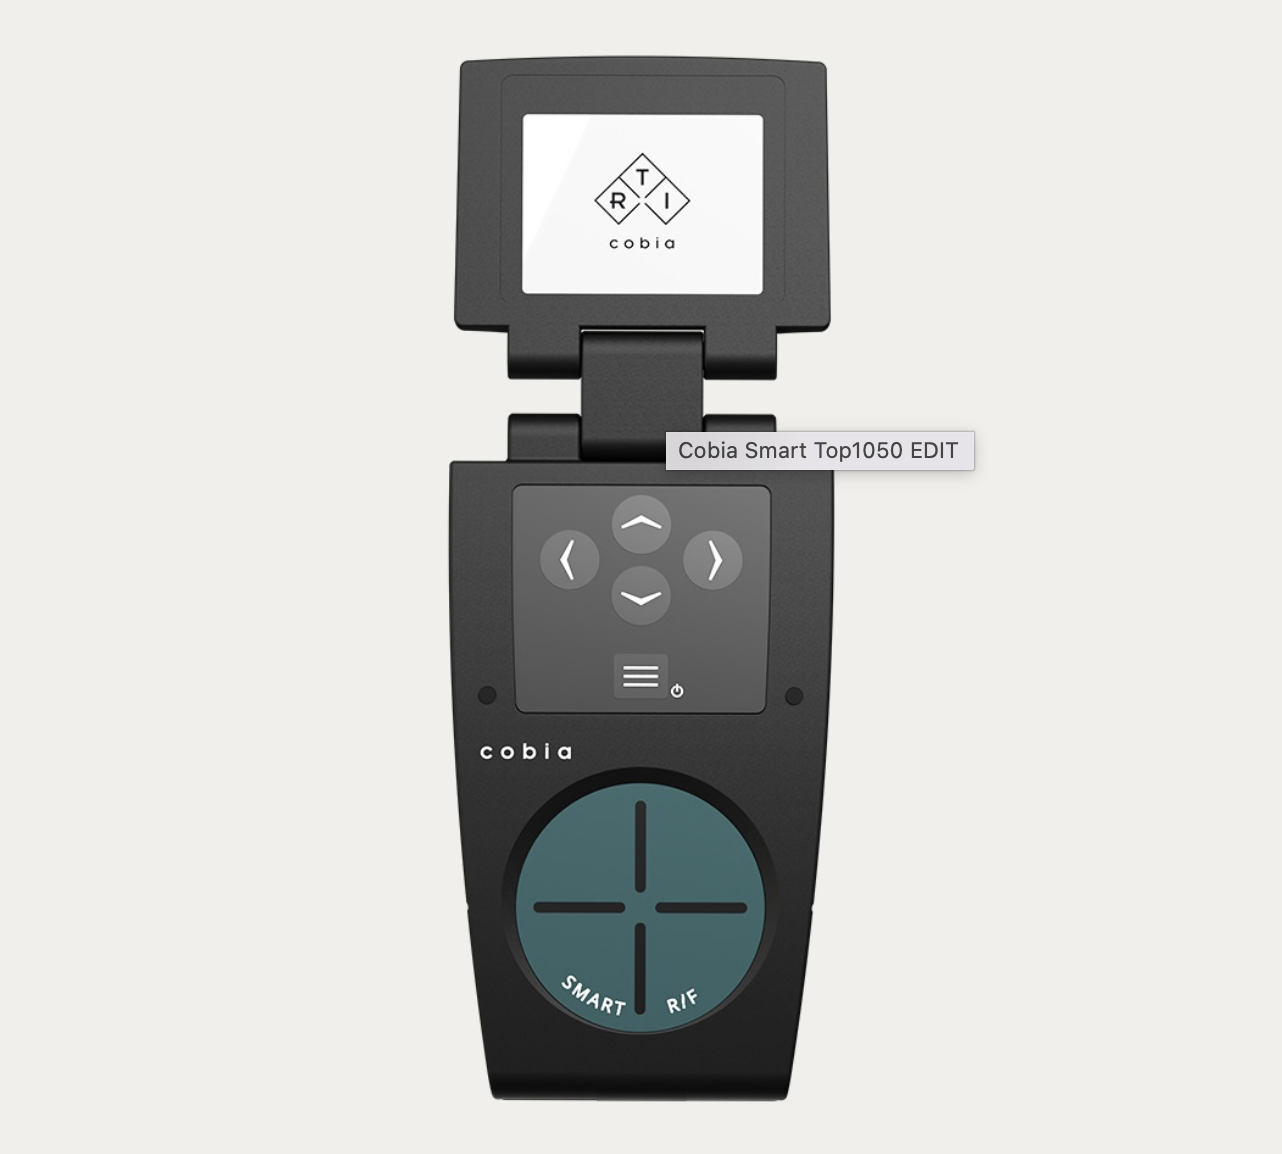
\includegraphics[width=\textwidth]{Figures/Theory_Figures/Cobia smart.png}
        \caption*{Cobia Smart R/F}
    \end{minipage}\hfill
    \begin{minipage}{0.32\textwidth}
        \centering
        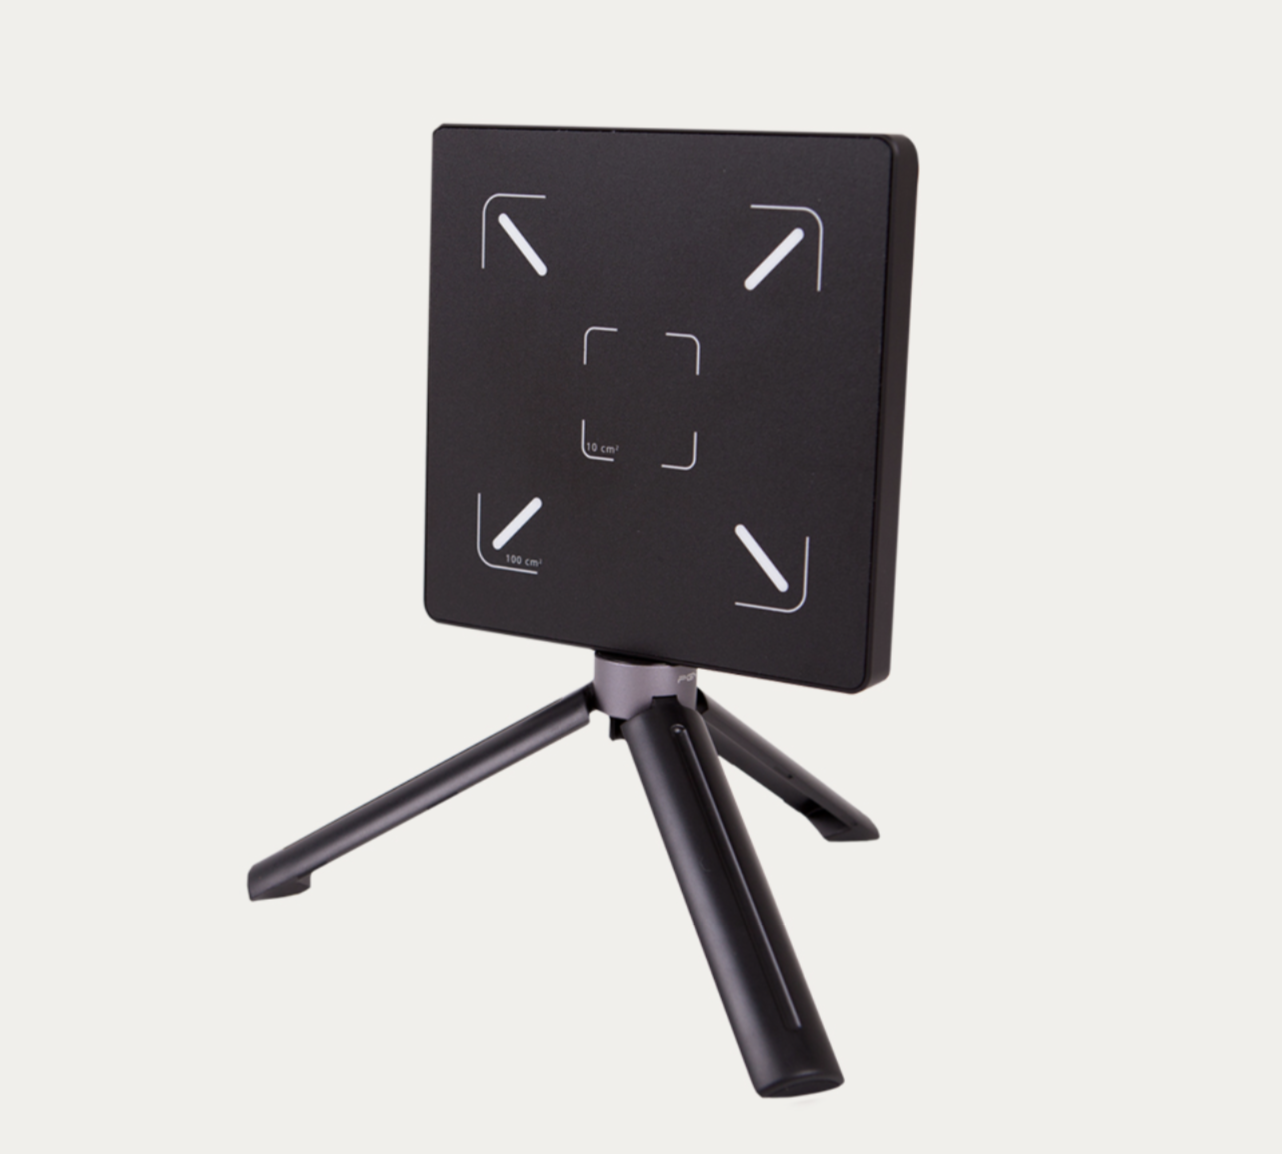
\includegraphics[width=\textwidth]{Figures/Theory_Figures/Scatter Probe.png}
        \caption*{RTI Scatter Probe}
    \end{minipage}\hfill
    \begin{minipage}{0.32\textwidth}
        \centering
        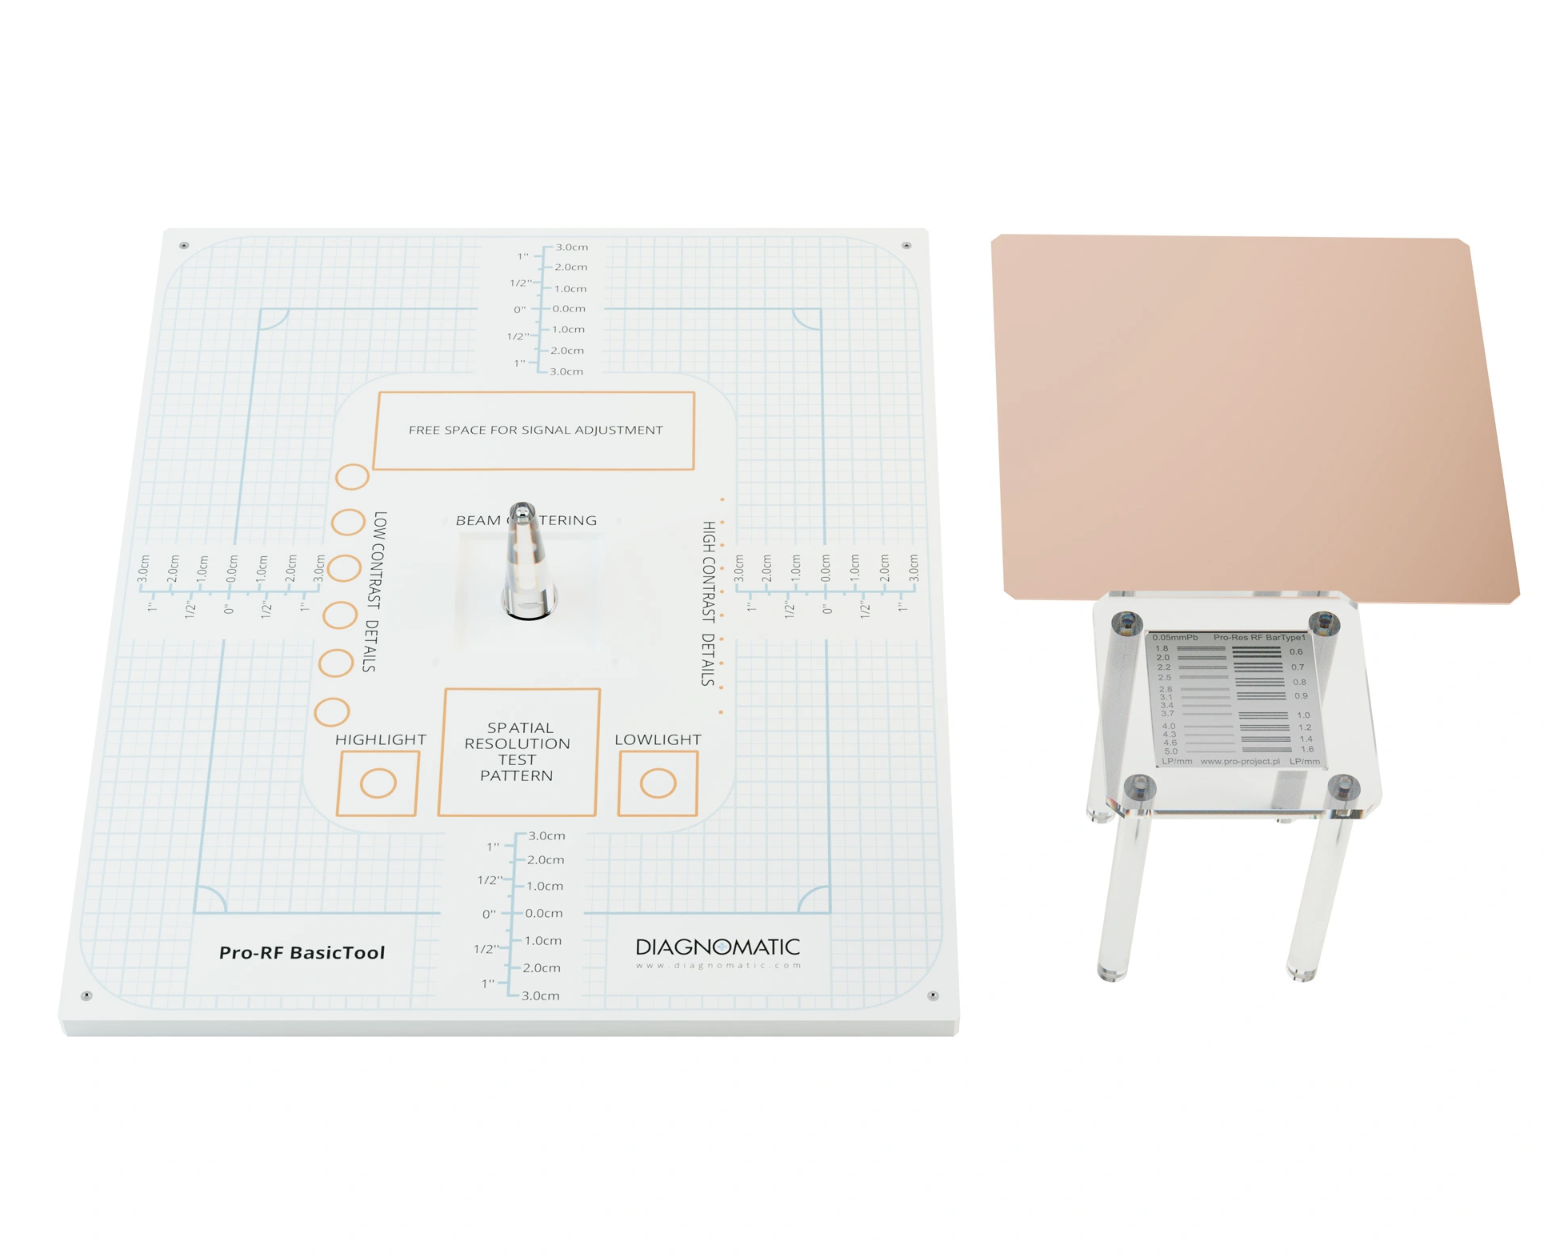
\includegraphics[width=\textwidth]{Figures/Theory_Figures/Pro_RFbasictool.png}
        \caption*{Pro-RF Basic tool}
    \end{minipage}
    \caption{X-Ray QA Kit Components}
\end{figure}

\subsection{The Pro-RF BasicTool phantom} 
The Pro-RF Basic tool is a quality assurance phantom designed for diagnostic X-ray machines. It is used to evaluate various parameters of X-ray imaging systems, including spatial resolution, contrast resolution, and image uniformity. The phantom typically consists of different test patterns and materials that simulate human tissue, allowing for comprehensive assessment of the imaging system's performance.

The Pro-RF Basic tool includes features such as:
\begin{itemize}
    \item outside dimensions: 345 $\times$ 290 mm
    \item high contrast array of 5 and 10 mm uniformly pitched mesh
    \item Highlight and Lowlight details
    \item 0.6 to 5.0 LP/mm resolution pattern
    \item 7$\times$ 11.0 mm diameter low contrast details
    \item 11$\times$ 0.5 mm diameter high contrast details
    \item extra stand for the spatial resolution pattern for focal spot size evaluation
    \item cone for perpendicular X-Ray beam control in the range of $0^o \div 1.5^o$
    \item an area of uniform attenuation suitable for noise measurements
    \item 1 mm Cu filter for HVL measurements    
\end{itemize}
